\documentclass{beamer}
\usepackage[utf8]{inputenc}
\usetheme{Boadilla}
\usecolortheme{dolphin}
\usepackage{lmodern}
\usefonttheme{professionalfonts}
\usepackage{amsmath,bm}
\usepackage{mathtools}
\usepackage{graphicx}
\usepackage{wrapfig}
\usepackage{hyperref}
\graphicspath{{figs/}}

\title[DeepONet]{DeepONet: Learning nonlinear operators for identifying differential equations based on the universal approximation theorem of operators}
\author[Lu]{\textbf{Lu Lu}, Pengzhan Jin, George Karniadakis}
\institute[Brown]{\normalsize{Division of Applied Mathematics, Brown University}}
\date[]{October 18, 2019}
\logo{
\includegraphics[height=1cm]{Brown.pdf}}

\begin{document}

\frame{\titlepage}

% \begin{frame}{Overview}
% \tableofcontents
% \end{frame}

\section{Introduction}

\begin{frame}{Introduction}
\begin{itemize}
\item Function: $\mathbb{R}^{d_1} \to \mathbb{R}^{d_2}$ \\
e.g., image classification:
\begin{tabular}{rl}
\begin{tabular}{r}

\includegraphics[height=1cm]{MNIST.png}
\end{tabular} &
\begin{tabular}{l}
\parbox{0.2\linewidth}{$\mapsto$ 5}
\end{tabular}
\end{tabular} \\
$\Rightarrow$ Neural network [Universal approximation theorem]
\vspace{2em} \pause
\item Operator: function ($\infty$-dim) $\mapsto$ function ($\infty$-dim) \\ \pause
e.g., derivative (local): $x(t) \mapsto x'(t)$ \\
e.g., integral (global): $x(t) \mapsto \int K(s,t) x(s)ds$ \\
e.g., dynamic system:
\begin{tabular}{l}
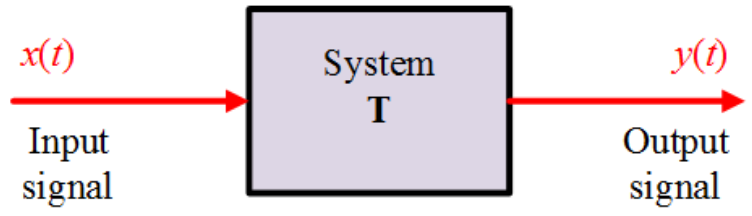
\includegraphics[height=1.25cm]{dynamic_system.png}
\end{tabular} \\ \pause
$\Rightarrow$ Can we learn operators via neural networks? \\
$\Rightarrow$ How?
\end{itemize}
\end{frame}

\begin{frame}{Problem setup}
$G: u \mapsto G(u)$ \\
$G(u): y \in \mathbb{R}^d \mapsto G(u)(y) \in \mathbb{R}$
\begin{figure}
\centering
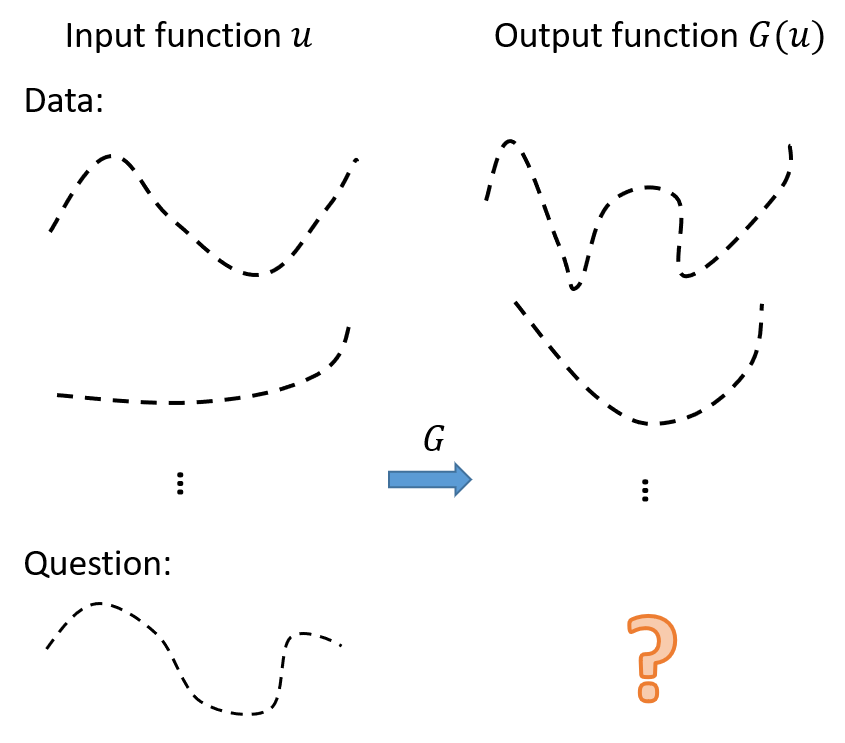
\includegraphics[width=7cm]{problem.png}
\end{figure}
\end{frame}

\begin{frame}{Network inputs and output}
$G: u \mapsto G(u)$ \\
$G(u): y \in \mathbb{R}^d \mapsto G(u)(y) \in \mathbb{R}$
\begin{itemize}
    \item Inputs: $u$ (\textcolor{red}{$\infty$-dim?}), $y \in \mathbb{R}^d$
    \item Output: $G(u)(y) \in \mathbb{R}$ \pause
    \item $u$ sensors: $x_1, x_2, \dots, x_m$
\end{itemize} \pause
\begin{figure}
\centering
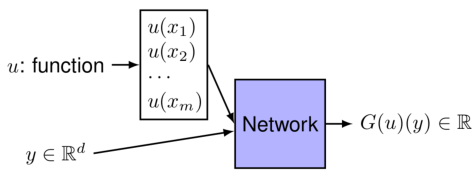
\includegraphics[width=8cm]{io.pdf}
\end{figure}
Assume $\{x_i\}$ ``dense'' enough, \\
is there a universal approximation theorem for operator?
\end{frame}

\begin{frame}{Universal Approximation Theorem for Operator}
$G: u \mapsto G(u)$, $G(u): y \in \mathbb{R}^d \mapsto G(u)(y) \in \mathbb{R}$
\begin{theorem}[Chen \& Chen, IEEE Trans. Neural Netw., 1995]
Suppose that $\sigma$ is a continuous non-polynomial function, $X$ is a Banach Space, $K_1 \subset X$, $K_2 \subset \mathbb{R}^d$ are two compact sets in $X$ and $\mathbb{R}^d$, respectively, $V$ is a compact set in $C(K_1)$, \textcolor{red}{$G$ is a nonlinear continuous operator}, which maps $V$ into $C(K_2)$. Then for any $\epsilon>0$, there are positive integers $n$, $p$, $m$, constants $c_i^k, \xi_{ij}^k, \theta_i^k, \zeta_k \in \mathbb{R}$, $w_k \in \mathbb{R}^d$, $x_j \in K_1$, $i=1,\dots,n$, $k=1,\dots,p$, $j=1,\dots,m$, such that
\begin{equation*}\label{eq:thm}
\left|\textcolor{red}{G(u)(y)} - \sum_{k=1}^p
\sum_{i=1}^n c_i^k \sigma\left(\sum_{j=1}^m \xi_{ij}^k \textcolor{red}{u(x_j)}+\theta_i^k\right)
\sigma(w_k \cdot \textcolor{red}{y}+\zeta_k)
\right|<\epsilon  
\end{equation*}
holds for all $u \in V$ and $y \in K_2$.
\end{theorem}
\end{frame}

\begin{frame}{Number of sensors}
Consider $G: u(x) \mapsto \boldsymbol{s}(x)$ ($x \in [0, 1]$) by ODE system
\begin{equation*}
\frac{d}{dx}\boldsymbol{s}(x)=\boldsymbol{g}(\boldsymbol{s}(x),u(x),x), \quad
\boldsymbol{s}(0)=\boldsymbol{s_0}
\end{equation*} \pause
\begin{tabular}{ll}
\begin{tabular}{l}
\parbox{0.3\linewidth}{$u\in V \Rightarrow u_m \in V_m$}
\end{tabular}
\begin{tabular}{l}
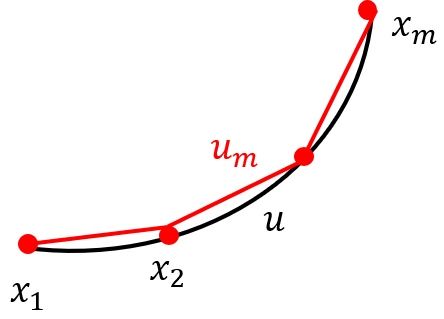
\includegraphics[height=2cm]{um.png}
\end{tabular} &
\end{tabular} \\ \pause
Let $\kappa(m,V) \coloneqq \sup_{u \in V} \max_{x\in[0,1]}|u(x)-u_m(x)|$ \\
e.g., Gaussian process with kernel $e^{- \frac{\| x_1 -x_2 \|^2}{2l^2}}$: $\kappa(m,V) \sim \frac{1}{m^2l^2}$
% \footnote{We thank Zhongqiang Zhang of Worcester Polytechnic Institute for the proof.}
\pause
\begin{theorem}[informal]
There exists a constant $C$, such that for any $y$,
\begin{equation*}
\sup_{u \in V} \|G(u)(y)- NN(u(x_1),\dots,u(x_m), y) \|_{2}< C\kappa(m,V).
\end{equation*}
\end{theorem}
\end{frame}

\begin{frame}
So far, we show
\begin{itemize}
\item operators can be approximated by neural networks
\item the number of sensors we need
\end{itemize}
\begin{figure}
\centering
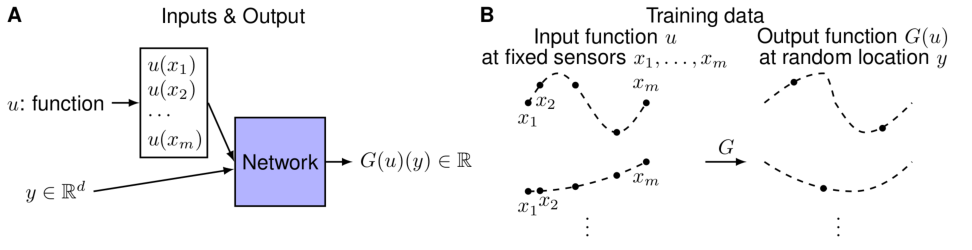
\includegraphics[width=.9\textwidth]{setup.pdf}
\end{figure} \pause
Q: How to design the network? \\
$\Rightarrow$ Deep operator network (DeepONet)
\end{frame}

\begin{frame}{DeepONet}
Recall the Theorem:
\begin{equation*}
G(u)(y) \approx \sum_{k=1}^p
\underbrace{\sum_{i=1}^n c_i^k \sigma\left(\sum_{j=1}^m \xi_{ij}^k \textcolor{red}{u(x_j)}+\theta_i^k\right)}_{branch}
\underbrace{\sigma(w_k \cdot \textcolor{red}{y}+\zeta_k)}_{trunk}
\end{equation*}
\begin{figure}
\centering
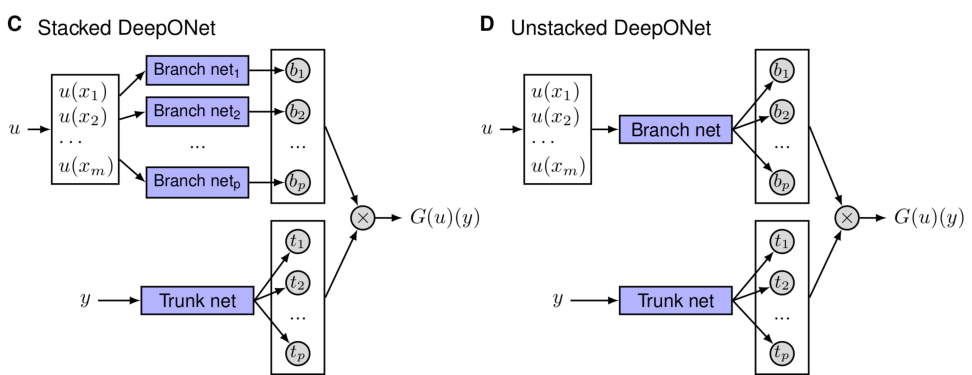
\includegraphics[width=.9\textwidth]{deeponet.pdf}
\end{figure}
\end{frame}

\begin{frame}{A simple ODE case}
$$\frac{ds(x)}{dx} = u(x), \quad x \in [0, 1],$$
with an initial condition $s(0)=0$.
$$G: u(x) \mapsto s(x) = \int_0^x u(\tau) d\tau$$ \pause
100 $u$ sensors, $10000 \textcolor{red}{\times 1}$ training points \\ \pause
Very small generalization error!
\begin{figure}
\centering
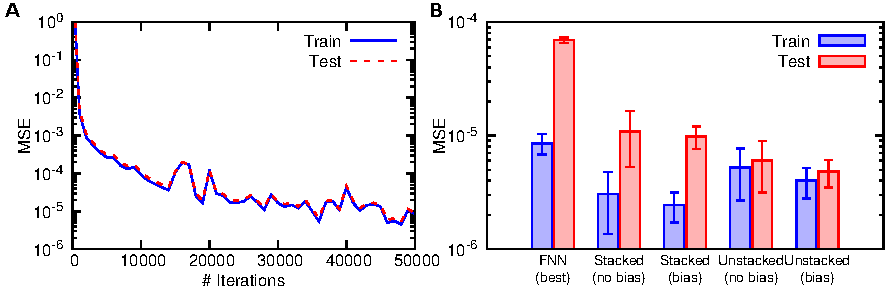
\includegraphics[width=.9\textwidth]{coefnet.pdf}
\end{figure}
\end{frame}

\begin{frame}{A nonlinear ODE case}
$$\frac{ds(x)}{dx} = -s^2(x) + u(x)$$ \pause
\begin{figure}
\centering
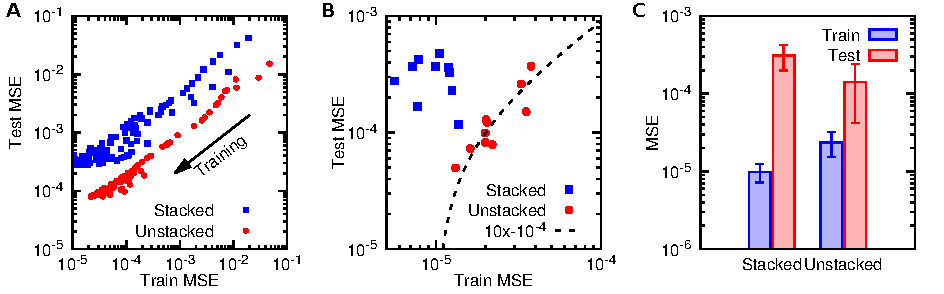
\includegraphics[width=.9\textwidth]{ode_stacked.pdf}
\end{figure}
Linear correlation between training and test errors
\begin{itemize}
\item A: in one training process \pause
\item B: across multiple runs (random dataset and network initialization)
\end{itemize}
\end{frame}

\begin{frame}{Gravity pendulum with an external force $u(t)$}
\begin{equation*}
\frac{ds_1}{dt} = s_2, \quad \frac{ds_2}{dt} = -k\sin s_1 + u(t)
\end{equation*}
\begin{figure}
\centering
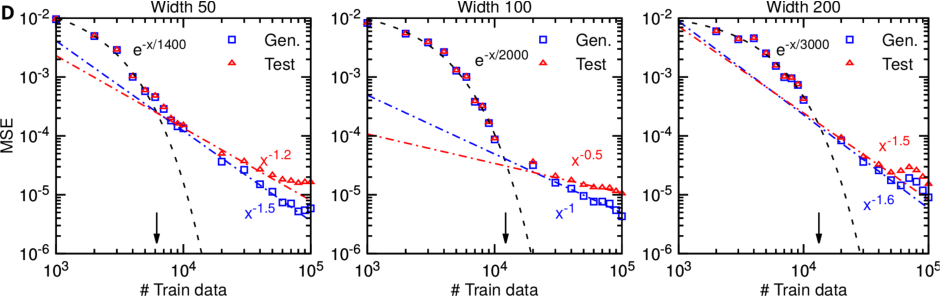
\includegraphics[width=.9\textwidth]{t.pdf}
\end{figure}
Test/generalization error:
\begin{itemize}
    \item small dataset: exponential convergence
    \item large dataset: polynomial rates
    \item smaller network has earlier transition point
\end{itemize}
\end{frame}

\begin{frame}{Diffusion-reaction system}
\begin{equation*}
    \frac{\partial s}{\partial t} = D\frac{\partial^2 s}{\partial x^2} + k s^2 + u(x), \quad x \in [0, 1], t \in [0, 1]
\end{equation*}
\begin{figure}
\centering
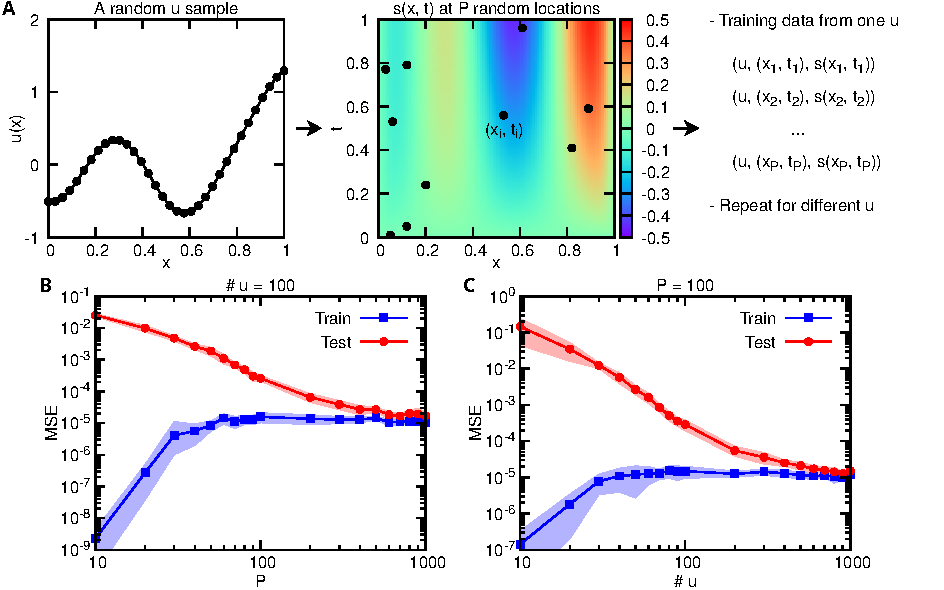
\includegraphics[width=.85\textwidth]{adr_error.pdf}
\end{figure}
\end{frame}

\begin{frame}{Diffusion-reaction system}
exponential/polynomial convergence
\begin{figure}
\centering
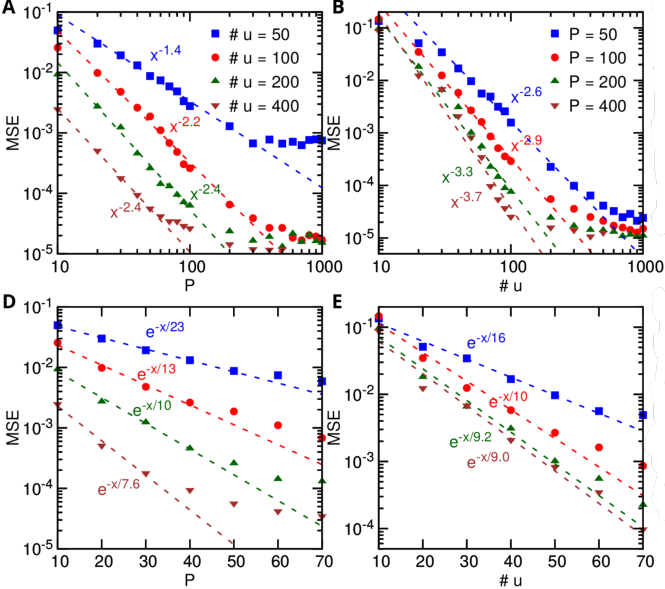
\includegraphics[width=.65\textwidth]{adr_convergence.pdf}
\end{figure}
\end{frame}

\begin{frame}{Summary}
\begin{itemize}
\item Number of sensors, $\kappa (m,V)$
\item DeepONet
\begin{itemize}
\item 1D ODE (linear, nonlinear), gravity pendulum, diffusion-reaction system (nonlinear)
\item Small generalization error
\item Exponential/polynomial error convergence
\end{itemize}
\end{itemize}
\vspace{1em}
\begin{itemize}
\item Lu, Jin, \& Karniadakis, arXiv:1910.03193, 2019.
\item DeepXDE: \url{https://deepxde.rtfd.io}
\end{itemize}
\end{frame}

\end{document}
